% TS-01 方法小结流程图 · 样张（全品导学案 p15 唯一处复刻）
% 参数依据：本目录 参数标定.txt（px→mm 口径 14.176px/mm）
% 说明句为自拟（登记见 简报.md）
\documentclass{article}
\usepackage[a4paper,left=18mm,right=18mm,top=22mm,bottom=20mm]{geometry}
\usepackage{fontspec}
\usepackage{xeCJK}
\setCJKmainfont{SimSun}
\setCJKfamilyfont{kai}{KaiTi}[AutoFakeBold=1.5]
\setCJKfamilyfont{hei}{SimHei}
\newcommand{\kaiti}{\CJKfamily{kai}}
\newcommand{\heiti}{\CJKfamily{hei}}
\usepackage{amsmath}
\usepackage{unicode-math}
\setmathfont{Cambria Math}
\newcommand{\vbi}[1]{\symbfit{#1}}
\usepackage{tikz}
\usetikzlibrary{shapes.geometric,arrows.meta,positioning}
\pagestyle{empty}
\setlength{\parindent}{2em}

\begin{document}
{\fontsize{10.5}{18.25}\selectfont
\heiti 【方法小结】空间向量模的坐标求法，按``先平方、再求和、后开方''三步进行。

\noindent 2．利用坐标法求向量模的步骤：

\vspace{2.4mm}
\begin{center}
% 显式坐标手绘（mm）：菱 16.1×9.1；矩 60.9×7.05 圆角1.3 左衬2.2；
% 横箭头 3.5；竖尖隙 3.2；行距（菱心距）12.3
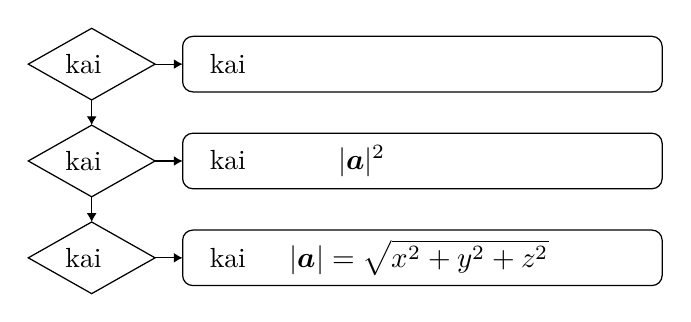
\begin{tikzpicture}[x=1mm,y=1mm,line width=0.45pt,
  fnt/.style={font=\kaiti\bfseries\fontsize{10.5}{12.6}\selectfont},
  ar/.style={-{Latex[length=3.2pt,width=3.6pt]}}]
  \foreach \y in {0,-12.3,-24.6}{
    \draw (8.05,\y) -- (0,\y+4.55) -- (-8.05,\y) -- (0,\y-4.55) -- cycle;
    \draw[rounded corners=1.3mm] (11.55,\y+3.525) rectangle (72.45,\y-3.525);
  }
  \node[fnt] at (0,0) {求模};
  \node[fnt] at (0,-12.3) {平方};
  \node[fnt] at (0,-24.6) {开方};
  \node[fnt,anchor=west] at (13.75,0) {将模的计算转化为坐标平方和};
  \node[fnt,anchor=west] at (13.75,-12.3) {代入坐标，求出平方和 $|\vbi{a}|^2$ 的值};
  \node[fnt,anchor=west] at (13.75,-24.6) {开方，得 $|\vbi{a}|=\sqrt{x^2+y^2+z^2}$};
  \draw[ar] (8.05,0) -- (11.55,0);
  \draw[ar] (8.05,-12.3) -- (11.55,-12.3);
  \draw[ar] (8.05,-24.6) -- (11.55,-24.6);
  \draw[ar] (0,-4.55) -- (0,-7.75);
  \draw[ar] (0,-16.85) -- (0,-20.05);
\end{tikzpicture}
\end{center}
}
\end{document}
